% !Mode:: "TeX:UTF-8"
% !TEX builder = LATEXMK
% !TEX program = xelatex
\documentclass[master,oneside]{zjuthesis} % 如果你的论文不满80页,还是单面印刷吧


%%%%%%%%%%%%%%%%%%%%%%%%%%%%%% 开始填写前置部分使用的变量
%%%%%%%%%%%%%%%%%%%%%%%%%%%%%% 样式设定在 zjuthesis.cls 下, 人类可读,爱请查阅

% 这里写这么鬼畜是为了测试多几个字会不会造成溢出
\title{这里写这么鬼畜是为了测试多几个字会不会造成溢出} % 封面和题名页使用
\englishtitle{The quick brown fox jumps over a lazy dog.The quick brown fox jumps over a lazy} % 封面和题名页使用,下划线三行,如果题目太短,去zjuthesis.cls 441 行微调
% 如果您的标题用字过多,请自行调节 zjuthesis.cls 里的 ZJUmakecover 里的各项距离。

\author{伊藤春希}          % 申请人姓名 封面使用

\classification{TP311.5}    % 封面头使用
\serialnumber{10335}        % 封面头使用
\secretlevel{无}            % 封面头使用
\studentnumber{21852xxx}    % 封面头使用

\supervisor{御坂美琴}       % 导师 封面使用
\spvtitle{电击使}           % 职称 封面使用

\cpsupervisor{桂和纱}       % 合作导师,如果没有合作导师,就在此文件第 4 行\documentclass选项栏中加上"nocpsupervisor"。
\cspvtitle{}             % 合作导师职称

% 从机械工程学院改来,保留设定变量命名
%\major{船舶工程}            % 专业学位类别栏 填 工程硕士
\major{工程硕士}
%\research{白学}             % 专业学位领域栏 填 软件工程
\research{软件工程}
\institute{软件学院}         % 所在学位栏 填 软件学院

\submitdate{2020年5月25日}   % 论文提交日期 栏 2333年2月33日

% 题名页的评阅人及答辩席
% 归档时候填写
% 论文评阅人1 2 3 4 5
\reviewerA{} \enreviewerA{}
\reviewerB{} \enreviewerB{}
\reviewerC{} \enreviewerC{}
\reviewerD{} \enreviewerD{}
\reviewerE{} \enreviewerE{}

% 答辩委员会主席
\chairperson{} \enchairperson{}

% 答辩委员 1 2 3 4 5
\commissionerA{} \encommissionerA{}
\commissionerB{} \encommissionerB{}
\commissionerC{} \encommissionerC{}
\commissionerD{} \encommissionerD{}
\commissionerE{} \encommissionerE{}

% 答辩日期
\defencedate{} \eendefencedate{}  % 因为endefencedate 命名被占用

% 论文前置部分变量填写完毕 开始全书排版
\begin{document}

% 封面、中文题名页、英文题名页、独创声明和版权使用书 无页码
\maketitle

% 摘要部分
\abstractmatter
% !TEX root = ../main.tex

% 定义中文摘要和关键字
\begin{cabstract}
请注意,以下内容主要参考自薛瑞尼的清华大学论文模板。

论文的摘要是对论文研究内容和成果的高度概括。
摘要应对论文所研究的问题及其研究\textbf{目的}进行描述,
对研究\textbf{方法和过程}进行简单介绍,
对研究\textbf{成果和所得结论}进行概括。
摘要应具有独立性和自明性,
其内容应包含与论文全文等量的主要信息。
使读者即使不阅读全文,
通过摘要就能了解论文的总体内容和主要成果。

论文摘要的书写应力求精确、简明。切忌写成对论文书写内容进行提要的形式,尤其要避
免“第 1 章……;第 2 章……;……”这种或类似的陈述方式。
不宜使用公式、图表,不标注引用文献。
硕士论文摘要的字数一般为300--500 个左右。

关键词是为了文献标引工作、
用以表示全文主要内容信息的单词或术语。
关键词不超过 5个,
每个关键词中间用分号分隔
(研究生院要求使用分号分隔,软件学院要求使用逗号分隔)。
见源码\texttt{zjuthesis.cls}搜索keywords了解。
\end{cabstract}

\ckeywords{\LaTeX, CJK, 模板, 毕业论文}
% !TEX root = ../main.tex

% 定义英文摘要和关键字

\begin{eabstract}
An abstract of a dissertation is a summary and extraction of research work
and contributions. Included in an abstract should be description of research
topic and research objective, brief introduction to methodology and research
process, and summarization of conclusion and contributions of the
research. An abstract should be characterized by independence and clarity and
carry identical information with the dissertation. It should be such that the
general idea and major contributions of the dissertation are conveyed without
reading the dissertation.

An abstract should be concise and to the point. It is a misunderstanding to
make an abstract an outline of the dissertation and words ``the first
chapter'', ``the second chapter'' and the like should be avoided in the
abstract.

Key words are terms used in a dissertation for indexing, reflecting core
information of the dissertation. An abstract may contain a maximum of 5 key
words, with semi-colons used in between to separate one another.
\end{eabstract}

\ekeywords{\TeX, \LaTeX, CJK, template, thesis}

% 目录和术语表
\frontmatter
\tableofcontents % 正文目录
\listoffigures   % 图目录
\listoftables    % 表目录
% 术语及缩略词表(需要则开)
%% !TEX root = ../proposal.tex
\begin{denotation}

\item[HPC] 高性能计算 (High Performance Computing)
\item[cluster] 集群
\item[Itanium] 安腾
\item[SMP] 对称多处理
\item[API] 应用程序编程接口
\item[PI]	聚酰亚胺
\item[MPI]	聚酰亚胺模型化合物,N-苯基邻苯酰亚胺
\item[PBI]	聚苯并咪唑
\item[MPBI]	聚苯并咪唑模型化合物,N-苯基苯并咪唑
\item[PY]	聚吡咙
\item[PMDA-BDA]	均苯四酸二酐与联苯四胺合成的聚吡咙薄膜均苯四酸二酐与联苯四胺合成的聚吡咙薄膜均苯四酸二酐与联苯四胺合成的聚吡咙薄膜
\item[$\Delta G$]  	活化自由能~(Activation Free Energy)
\item [$\chi$] 传输系数~(Transmission Coefficient)
\item[$E$] 能量
\item[$m$] 质量
\item[$c$] 光速
\item[$P$] 概率
\item[$T$] 时间
\item[$v$] 速度
\end{denotation}


% 正文排版开始 建议一章一文件 (好像无法嵌套 include) 
\mainmatter
% !TEX root = ../proposal.tex

\chapter{绪论\texorpdfstring{\footnote{章标题中脚注命令测试}}{}(or 引言)各种测试}
绪论占坑,但是也要测试到底占多少缩进,换行情况,行距,都是这些不听话的小伙伴,好好调教你们。

\section{列表环境\texorpdfstring{\footnote{节标题中脚注命令测试}}{}测试}
以下是一个测试用的列表环境,内容不要在意。\footnote{正文中中脚注命令测试,长脚注情况:这包括如下事实:“未经本人同意,监听、录制或转播私人性质的谈话或秘密谈话;未经本人同意,拍摄、录制或转播个人在私人场所的形象”}

这里测试列表标签功能的交叉引用格式\ref{itm:11},\ref{itm:12},\ref{itm:13},\ref{itm:14},分别表示第一至第四层级的itemize系列的交叉引用情况。
\begin{enumerate}
	\item 第一级列表\label{itm:11}
	\item 第一级列表
	\begin{enumerate}
		\item 第二级列表\label{itm:12}
		\item 第二级列表
		\begin{enumerate}
			\item 第三级列表\label{itm:13}
			\item 第三级列表
			\begin{enumerate}
				\item 第四级列表\label{itm:14}
				\item 第四级列表
				\item 第四级列表
				\item 第四级列表
			\end{enumerate}
			\item 第三级列表
			\item 第三级列表
			\item 第三级列表
		\end{enumerate}
		\item 第二级列表
		\item 第二级列表
	\end{enumerate}
	\item 第一级列表
	\item 第一级列表
	\item 第一级列表
\end{enumerate}

正是由于油膜物质的发现,使“雾伞”计划成为可能,这个计划是用核爆炸在太空中蒸发和扩散油膜物质,在太阳与地球之间形成一团“油膜尘埃”,降低太阳 对地球的辐射,达到缓解地球温室效应的目的。“我记得,海王星轨道附近应该还有前战争时期的恒星型核弹吧?”肯又问。“有的,‘雾伞’工程的飞船也装载了一些,在海王星环和卫星上爆破用,具体数目不清楚。” “好像一颗就够了。”肯兴奋起来。两个世纪前面壁者雷迪亚兹的战略计划中所研制的恒星型氢弹,后来共制造了五千多颗。虽然这种武器在末日之战中作用有限,但正如雷迪亚兹所言,各大 国主要是为可能爆发的人类之间的行星际战争准备的,核弹主要在大低谷时期制造,那时由于资源的匮乏,国际关系极其紧张,人类自身的战争一触即发。进入新时期后,这些骇人听闻的武器成了危险的鸡肋,虽然其所有权都属于地球国家, 但还是都被送入太空存贮,少部分已经用于行星工程的爆破,还有一部分送入太阳系外围轨道。曾有人设想将核弹中的聚变材料可以作为远程飞船的燃料补充,但由于核弹的拆解很困难,这个设想一直没有真正实现过\footnote{看看另起一页脚注编号的变化}。
\begin{itemize}
	\item 第一级列表
	\item 第一级列表
	\begin{itemize}
		\item 第二级列表
		\item 第二级列表
		\begin{itemize}
			\item 第三级列表
			\item 第三级列表
			\begin{itemize}
				\item 第四级列表
				\item 第四级列表
				\item 第四级列表
				\item 第四级列表
			\end{itemize}
			\item 第三级列表
			\item 第三级列表
			\item 第三级列表
		\end{itemize}
		\item 第二级列表
		\item 第二级列表
	\end{itemize}
	\item 第一级列表
	\item 第一级列表
	\item 第一级列表
\end{itemize}

“你觉得能行,”罗宾逊两眼放光地问道,他后悔这么简单的事自己怎么没 想到,一个载入史册的机会让肯抢去了。“试试吧,只有这一个办法了。”“如果行,博士,以后林格一斐兹罗监测站将永远按产生1G重力的速度旋转。”“这可是人类造出来的最大的东西了。”“蓝影”号飞船的指令长看着舱外漆黑的太空说,他极力想象自己能看到尘埃云,但确实什么\footnote{连续两个脚注测试1}\footnote{连续两个脚注测试2}
\begin{enumerate}
	\item 第四级列表
	\item 第四级列表
	\begin{enumerate}
		\item 第五级列表
		\item 第五级列表
		\item 第五级列表
	\end{enumerate}
	\item 第四级列表
	\item 第四级列表
\end{enumerate}
都看不到。“为什么它不能被阳光照出来呢,就像彗星的尾巴那样...”飞船驾驶员说,“蓝影”号上只有他和指令长两个人。他知道,尘埃云的密度确实像彗星尾一样稀薄,几乎和地球上实验室中造出的真空差不多。“可能是阳光太弱吧。”指令长回头看看太阳,在这海王星轨道和柯伊伯带 之间的冷寂空间,太阳看上去只是一颗刚能看出圆盘形状的大星星。阳光倒是还可以在舱壁上照出亮影,但已经十分微弱了。“再说,彗尾也要在一定的距离外 才能看到,我们可是就在云的边缘。”

\section{参考文献测试}
测试一下引用\cite{shi_chinas_2010},引用\cite{shi2010china,hata2014soi,muhammad2011development},还有其它引用\cite{shi2010china,muhammad2011development,lamport1994latex}.

\section{浮动体测试}
\subsection{插图测试}
如\autoref{fig:first_image_tset}是对此模版的第一张插图测试。

\begin{figure}[htbp]
	\centering
	
\includegraphics[width = 0.5\linewidth]{Chapter1.png}
	\bicaption{第一张插图测试\cite{texbook}}{The first picture test}
	\label{fig:first_image_tset}
\end{figure}

以下是一段对这些插图来历的介绍,引用自知乎专栏All about TeXnique中夏晓昊的文章\href{http://zhuanlan.zhihu.com/LaTeX/19669122}{《The TeXbook导读:从那头(多图杀猫的)狮子说起》}。

在The TeXbook中,有着一系列的以狮子为主题的插图。这些插图的作者是Duane Bibby。也是从The TeXbook开始,不少TeX书也采取了以狮子为主的插图,作者也是Duane Bibby。另外,每年的TUG(TeX Users Group)年会都会有一张以狮子为主题的logo,这只狮子已经是社区的吉祥物了。

为什么选择狮子呢?Yannis Haralambous写道(原文法语,此为转译后的英文):Not for nothing is TeX represented by a lion. Donald Knuth has told us that lions are to him the guardians of libraries in the United States because there is a statue of a lion in front of the entrance of each large library there. Guardian of libraries, guardian of the Book—is that not indeed what TeX ultimately aspires to be? 或许吧。 (顺便说一句,TeX和MetaFont都用了狮子,TeX是公狮子,MetaFont是母狮子,多么和谐的一对啊。如果你还是忽略MetaFont的存在,那你还没有认识到它的重要性。)

作为插图,首要的一点就是贴切,然后是有趣。在TeX社区里面,have fun是一个很重要的词组,也有人说Happy TeXing。我知道有不少人不喜欢TeX,但是能有什么理由呢?如果你用不到它,那么浅尝辄止即可。如果你会用到很频繁,最好慢慢修炼做到精通。如果你只是偶尔用到,那么可以搬个模版什么的,甚至也可以找人帮你(不要指望别人会用足够的空闲时间来帮你,他没有这个义务,请支付报酬,最少也得请吃个红烧肉吧)。下面的插图,是TeX TeXbook中的,我也希望这个新年的假期,能有人有空来看看这本书。即使不能把所有的东西都看懂,那么也会对TeX的设计有了一定的了解,拿到扳手就好。

\subsection{表格测试}
在这里推荐制表采用功能强大的tabu宏包以取代其它制表宏包。具体tabu宏包的使用说明参见tabu宏包的说明文档。

以下节分别用来测试各种表格环境如,tabular,tabu,longtabu等,还有对caption格式的修改和测试。以下表格样式全部采用三线表。

\subsubsection{array宏包tabular表格环境测试}
如\autoref{tab:first_table_test}是对array宏包的tabular表格环境测试。
\begin{table}[htbp]
	\centering
	\bicaption{这是一个用tabular环境的测试用的表格}{The first table}\label{tab:first_table_test}
    \begin{tabular}{lrr}
    \toprule
    \textbf{行星}     & \textbf{赤道半径}km & \textbf{公转周期}d \\
    \midrule
    水星     & 2.439  & 87.9 \\
    金星     & 6.1    & 224.682 \\
    地球     & 6378.14 & 365.24 \\
    \bottomrule
    \end{tabular}%
\end{table}

\subsubsection{tabu宏包表格环境测试}
如\autoref{tab:tabu_test_1}是对tabu宏包的tabu表格环境测试。在这里表格命令与\autoref{tab:first_table_test}的命令相同,只是tabular环境改成了tabu环境。
\begin{table}[htbp]
	\centering
	\bicaption{这是一个用tabu环境的测试用的表格}{bicaption in tabu enviroment}\label{tab:tabu_test_1}
    \begin{tabu}{lrr}
    \toprule
    \textbf{行星}     & \textbf{赤道半径}km & \textbf{公转周期}d \\
    \midrule
    水星     & 2.439  & 87.9 \\
    金星     & 6.1    & 224.682 \\
    地球     & 6378.14 & 365.24 \\
    \bottomrule
    \end{tabu}%
\end{table}

\autoref{tab:tabu_test_2}对tabu to表格的x列模式进行测试。在表格导言区中设置为X[1]X[2]X[2],表示这三列表格的列宽比值为1:2:2,总的表格宽度由tabu to环境设置,这里设置为0.6\textbackslash linewidth。相比于tabular环境,tabu环境的列宽设置方便许多。
\begin{table}[htbp]
	\centering
	\caption{tabu环境测试表格---X列模式}\label{tab:tabu_test_2}
    \begin{tabu} to 0.6\linewidth{X[1]X[2]X[2]}
    \toprule
    \textbf{行星}     & \textbf{赤道半径}km & \textbf{公转周期}d \\
    \midrule
    水星     & 2.439  & 87.9 \\
    金星     & 6.1    & 224.682 \\
    地球     & 6378.14 & 365.24 \\
    \bottomrule
    \end{tabu}%
\end{table}

如\autoref{tab:tabu_test_3}是longtabu环境测试表格。longtabu环境不能用在table浮动体环境中。根据GB/T 7713.1-2006规定:如果某个表需要转页接排,在随后的各页上应重复表的编号。编号后跟标题(可省略)和“(续)”,置于表上方。续表应重复表头。

特别需要注意的是,longtabu是基于longtable宏包开发的,所以在zjuthesis.cls文件中已经插入了longtable宏包。longtable环境的所有功能都可以在longtabu中使用,如\textbackslash endhead,\textbackslash endfirsthead,\textbackslash endfoot,\textbackslash endlastfoot,和\textbackslash caption等。具体用法请参见longtable和tabu宏包的相应文档。
\begin{longtabu}{lccc}
\bicaption{材料弹性模量及泊松比}{bicaption in longtable}\label{tab:tabu_test_3}\\
\toprule
名  称   & 弹性模量E/Gpa & 切变模量G/Gpa & 泊松比$\mu$ \\
\midrule%
\endfirsthead
\caption{材料弹性模量及泊松比(续)}\\
\toprule
名  称   & 弹性模量E/Gpa & 切变模量G/Gpa & 泊松比$\mu$ \\
\midrule%
\endhead
\bottomrule%
\endfoot
镍铬钢、合金钢 & 206    & 79.38  & 0.3 \\
碳 钢    &  196~206 & 79     & 0.3 \\
铸 钢    &  172~202 &        & 0.3 \\
球墨铸铁   &  140~154 &  73~76 & 0.3 \\
灰铸铁、白口铸铁 &  113~157 & 44     &  0.23~0.27 \\
冷拔纯铜   & 127    & 48     &   \\
轧制磷青铜  & 113    & 41     &  0.32~0.35 \\
轧制纯铜   & 108    & 39     &  0.31~0.34 \\
轧制锰青铜  & 108    & 39     & 0.35 \\
铸铝青铜   & 103    & 41     & 0.3 \\
冷拔黄铜   &  89~97 &  34~36 &  0.32~0.42 \\
轧制锌    & 82     & 31     & 0.27 \\
硬铝合金   & 70     & 26     & 0.3 \\
轧制铝    & 68     &  25~26 &  0.32~0.36 \\
铅      & 17     & 7      & 0.42 \\
玻璃     & 55     & 22     & 0.25 \\
混凝土    &  14~39 &  439~15.7 &  0.1~0.18 \\
纵纹木材   &  9.8~12 & 0.5    &   \\
横纹木材   &  0.5~0.98 &  0.44~0.64 &   \\
橡胶     & 0.00784 &        & 0.47 \\
电木     &  1.96~2.94 &  0.69~2.06 &  0.35~0.38 \\
赛璐珞    &  1.71~1.89 &  0.69~0.98 & 0.4 \\
可锻铸铁   & 152    &        &  \\
拔制铝线   & 69     &        &  \\
大理石    & 55     &        &  \\
花岗石    & 48     &        &  \\
石灰石    & 41     &        &  \\
尼龙1010 & 1.07   &        &  \\
夹布酚醛塑料 &  4~8.8 &        &  \\
石棉酚醛塑料 & 1.3    &        &  \\
高压聚乙烯  &  0.15~0.25 &        &  \\
低压聚乙烯  &  0.49~0.78 &        &  \\
聚丙烯    &  1.32~1.42 &        &  \\
硬聚氯乙烯  &  3.14~3.92 &        &  \\
聚四氟乙烯  &  1.14~1.42 &        &  \\
\end{longtabu}%

\subsection{子图}
这里子图的排版推荐使用subcaption宏包,不再推荐使用subfig宏包,更不推荐使用subfigure宏包。值得注意的是,在zjuthesis.cls文件中已经写入了subcaption宏包,而且subcaption宏包与subfigure和subfig宏包是相互冲突的。因此,如果你还想使用subfig宏包而不想使用subcaption宏包,请自己到zjuthesis.cls文件的相关位置更改,具体的使用及修改方法参见相应的宏包说明文档。不过在这里还是不推荐直接去更改zjuthesis.cls文档,除非你对\LaTeX 的相关命令很清楚,知道自己在改什么,并且不会对其他格式产生影响。

具体的subcaption宏包使用方法我这里不仔细介绍,以下只是对subcaption进行一些简单的测试,主要是格式调整和交叉引用。

如\autoref{fig:subfig_test1}是有两张子图的模式,对子图进行交叉引用,如\autoref{subfig:1a}和\autoref{subfig:1b}。

\begin{figure}[htbp]
	\centering
	\begin{subfigure}[b]{.4\textwidth}
		\centering
		
\includegraphics[width = \textwidth]{Chapter2.png}
		\bisubcaption{书籍排版与普通排版}{bicaption in subcaption}\label{subfig:1a}
	\end{subfigure}
	\quad
	\begin{subfigure}[b]{.4\textwidth}
		\centering
		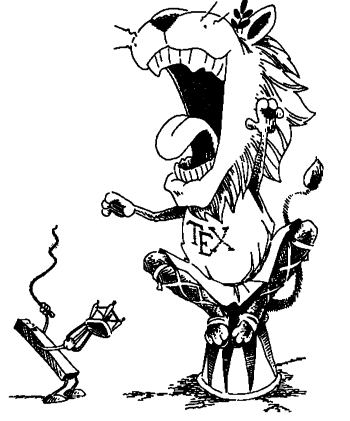
\includegraphics[width = \textwidth]{Chapter3.png}
		\caption{\TeX 的控制系列}\label{subfig:1b}
	\end{subfigure}
	\bicaption{子图模式测试1:2张图}{bicaption in subfigure}\label{fig:subfig_test1}
\end{figure}

如\autoref{fig:subfig_test2}是有四张子图的模式,对子图进行交叉引用,如\autoref{subfig:2a}、\autoref{subfig:2b}、\autoref{subfig:2c}和\autoref{subfig:2d}。

\begin{figure}[htbp]
	\centering
	\begin{subfigure}[b]{.4\textwidth}
		\centering
		
\includegraphics[width = \textwidth]{Chapter4.png}
		\caption{字体}\label{subfig:2a}
	\end{subfigure}
	\begin{subfigure}[b]{.4\textwidth}
		\centering
		
\includegraphics[width = \textwidth]{Chapter5.png}
		\caption{编组}\label{subfig:2b}
	\end{subfigure}
	\begin{subfigure}[b]{.4\textwidth}
		\centering
		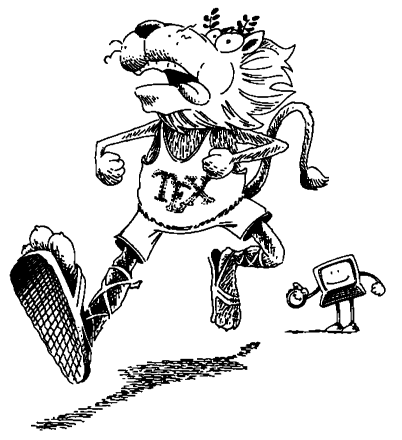
\includegraphics[width = \textwidth]{Chapter6.png}
		\caption{运行\TeX}\label{subfig:2c}
	\end{subfigure}
	\begin{subfigure}[b]{.4\textwidth}
		\centering
		
\includegraphics[width = \textwidth]{Chapter7.png}
		\caption{\TeX 工作原理}\label{subfig:2d}
	\end{subfigure}
	\caption{子图模式测试2:4张图}\label{fig:subfig_test2}
\end{figure}

\subsection{数学模式测试}
数学模式测试,主要测试数学字体,编号和交叉引用。这里首先推荐使用\texttt{align}和\texttt{align*}数学模式环境,大多数行间数学模式只需要用这个环境就可以了。

交叉引用测试,如交引用命令{\ttfamily \textbackslash eqref}和\texttt{\textbackslash ref}命令的区别。如公式\eqref{eq:test1},公式\ref{eq:test1}显示,\texttt{\textbackslash eqref}命令比\texttt{\textbackslash ref}命令的应用结果多了个括号。

如公式\eqref{eq:test3}是单行公式环境,查看公式\eqref{eq:test3}和\eqref{eq:test1}之间的区别,好像在单行公式中没什么区别。
\begin{align}\label{eq:test3}
	f(x) = 2(x + 1)^{2} - 1
\end{align}

\texttt{align}公式环境,用在单行中。
\begin{align}\label{eq:test1}
	f(x) = 2(x + 1)^{2} - 1
\end{align}

在这里,中间插入一些文字以形成段落,查看行间公式与上下文之间的间隙。
\begin{align*}
	f(x) = 2(x + 1)^{2} - 1
\end{align*}
在这里,中间插入一些文字以形成段落,查看行间公式与上下文之间的间隙。下一个公式\eqref{eq:test2}是一个公式组,它在“=”位置对齐。
\begin{align}\label{eq:test2}
	f(x) & = 2(x + 1)^{2} - 1\\
		 & = 2(x^{2} + 2x +1)-1\\
		 & = 2x^{2} + 4x + 1
\end{align}


\section{关于引用}
图表的引用通过{\ttfamily \textbackslash autoref} 命令即可,使用ST LaTeXTools 插件还能自动补全。如果要修改前缀,那么就用{\ttfamily \textbackslash recnewcommand \textbackslash figureautorefname\{好图\}}即可,详见hyperref宏包说明。

\section{出现的问题}
\subsection{\textbackslash texttt}
在这里发现一个问题,在下面的例子中可以发现,在中文中使用\textbackslash texttt\{\}命令时,前面的汉字与接下来的英文单词的空隙明显比接下来单词跟汉字的间隙要大,但是其它命令没有什么问题。

\begin{center}
\noindent 问题\texttt{问题}问题,问题\textbackslash\texttt{问题}问题。\\
问题\texttt{ref} 问题,问题\texttt{\textbackslash ref} 问题。\\
问题\textbf{ref}问题,问题\textbf{\textbackslash ref}问题。\\
问题\textsf{ref}问题,问题\textsf{\textbackslash ref}问题。\\
problem \texttt{ref} problem,problem \texttt{\textbackslash ref} problem.\\
problem \textbf{ref} problem,problem \textbf{\textbackslash ref} problem.\\
problem \textsf{ref} problem,problem \textsf{\textbackslash ref} problem.
\end{center}

原来的编译环境为texlive 2014,编译环境改为texlive 2015后,问题解决。
 % 绪论
\include{contents/sample/whyla}
\include{contents/sample/elem}
\include{contents/sample/sum}

% 结尾部分排版
\backmatter

% 引用参考文献数据库
\bibliography{references/test.bib}

% 附录部分
%\appendix
%% !TEX root = ../proposal.tex
\chapter{我是第一个附录}
\section{我是第一个附录的第一节}
这是一个附录测试页,内容无关紧要。\footnote{以下内容引用自《三体:黑暗森林》}以%
下段落较长,以防数组溢出,故采用回车强制分行处理。分行出换行符在\TeX 中算作一个%
空格,因此,在每段后加注释符。不过在中文环境中换行加不加注释符都不会产生空格,不%
过还是加上吧。

罗辑抬起左手,露出了戴在手腕上的手表大小的东西说:“这是一个生命体征监测仪,它通%
过一个发射器与一套摇篮系统联结。你们一定记得两个世纪前面壁者雷迪亚兹的事,那就一%
定知道摇篮系统是什么。这个监测仪所发出的信号通过摇篮系统的链路,到达雪地工程部署%
在太阳轨道上的三千六百一十四枚核弹。

信号每秒钟发射一次,维持着这些核弹的非触发状态。如果我死去,摇篮系统的维持信号将%
消失,所有的核弹将被引爆,包裹核弹的油膜物质将在爆炸中形成围绕太阳的三千六百一十%
四团星际尘埃,从远方观察,在这些尘埃云团的遮挡下,太阳将在可见光和其他高频渡段发%
生闪烁。太阳轨道上所有核弹的位置都是经过精心布置的,使得太阳闪烁形成的信号发送出%
三张简单的图形,就像我两个世纪前发出的那三张图一样,每张上面有三十个点的排列,并%
标注其中一个点,它们可以组合成一个三维坐标图。但与那次不同的是,这次发送的,是三%
体世界与周围三十颗恒星的相对位置。太阳将变成银河系中的一座灯塔,把这咒语发送出去%
,当然,太阳系和地球的位置也会同时暴露。从银河系中的一点看,图形发射完成需要一年%
多的时间,但应该有很多技术发展到这样程度的文明,可以从多个方向同时观测太阳,那样%
的话,只需几天甚至几个小时,他们就能得到全部信息。”

\section{数学模式测试}
这里用于测试附录部分的数学公式,诸如标号,交叉应用等。

交叉引用测试,如交引用命令{\ttfamily \textbackslash eqref}和\texttt{\textbackslash ref}命令的区别。如公式\eqref{eq:apptest1},\autoref{eq:apptest1}显示,\texttt{\textbackslash eqref}命令比\texttt{\textbackslash ref}命令的应用结果多了个括号。

如公式\eqref{eq:apptest3}是单行公式环境,查看公式\eqref{eq:apptest3}和\eqref{eq:apptest1}之间的区别,好像在单行公式中没什么区别。
\begin{align}\label{eq:apptest3}
	f(x) = 2(x + 1)^{2} - 1
\end{align}

\texttt{align}公式环境,用在单行中。
\begin{align}\label{eq:apptest1}
	f(x) = 2(x + 1)^{2} - 1
\end{align}

在这里,中间插入一些文字以形成段落,查看行间公式与上下文之间的间隙。
\begin{align*}
	f(x) = 2(x + 1)^{2} - 1
\end{align*}
在这里,中间插入一些文字以形成段落,查看行间公式与上下文之间的间隙。下一个公式\eqref{eq:apptest2}是一个公式组,它在“=”位置对齐。
\begin{align}\label{eq:apptest2}
	f(x) & = 2(x + 1)^{2} - 1\\
		 & = 2(x^{2} + 2x +1)-1\\
		 & = 2x^{2} + 4x + 1
\end{align}

\subsection{我是第一个附录的第二节的第一个子节}

\section{表格测试}
在这里推荐制表采用功能强大的tabu宏包以取代其它制表宏包。具体tabu宏包的使用说明参见tabu宏包的说明文档。

以下节分别用来测试各种表格环境如,tabular,tabu,longtabu等,还有对caption格式的修改和测试。以下表格样式全部采用三线表。

\subsection{array宏包tabular表格环境测试}
如\autoref{tab:appfirst_table_test}是对array宏包的tabular表格环境测试。
\begin{table}[htbp]
	\centering
	\caption{这是一个用tabular环境的测试用的表格}\label{tab:appfirst_table_test}
    \begin{tabular}{lrr}
    \toprule
    \textbf{行星}     & \textbf{赤道半径}km & \textbf{公转周期}d \\
    \midrule
    水星     & 2.439  & 87.9 \\
    金星     & 6.1    & 224.682 \\
    地球     & 6378.14 & 365.24 \\
    \bottomrule
    \end{tabular}%
\end{table}

\subsection{tabu宏包表格环境测试}
如\autoref{tab:apptabu_test_1}是对tabu宏包的tabu表格环境测试。在这里表格命令与\autoref{tab:appfirst_table_test}的命令相同,只是tabular环境改成了tabu环境。
\begin{table}[htbp]
	\centering
	\caption{这是一个用tabu环境的测试用的表格}\label{tab:apptabu_test_1}
    \begin{tabu}{lrr}
    \toprule
    \textbf{行星}     & \textbf{赤道半径}km & \textbf{公转周期}d \\
    \midrule
    水星     & 2.439  & 87.9 \\
    金星     & 6.1    & 224.682 \\
    地球     & 6378.14 & 365.24 \\
    \bottomrule
    \end{tabu}%
\end{table}

\section{插图测试}
如\autoref{fig:appfirst_image_tset}是对此模版的第一张插图测试。

\begin{figure}[htbp]
	\centering
	
\includegraphics[width = 0.5\linewidth]{Chapter8.png}
	\caption{附录页第一张插图测试}\label{fig:appfirst_image_tset}
\end{figure}

\section{我是第一个附录的第五节}
随着天光渐明,星星在一颗颗消失,仿佛无数只眼睛渐次闭上;而东方正在亮起的晨空,则%
像一只巨大的眼睛在慢慢睁开。蚂蚁继续在叶文洁的墓碑上攀爬着,穿行在她的名字构成的%
迷宫中。早在这个靠碑而立的豪赌者出现前的一亿年,它的种族已经生活在地球上,这个世%
界有它的一份,但对正在发生的事,它并不在意。

罗辑离开墓碑,站到他为自己挖掘的墓穴旁,将手枪顶到自己的心脏位置,说:“现在,我
将让自己的心脏停止跳动,与此同时我也将成为两个世界有史以来最大的罪犯。对于所犯下
的罪行,我对两个文明表示深深的歉意,但不会忏悔,因为这是唯一的选择。我知道智子就
在身边,但你们对人类的呼唤从不理睬,无言是最大的轻蔑,我们忍受这种轻蔑已经两个世
纪了,现在,如果你们愿意,可以继续保持沉默,我只给你们三十秒钟时间。”罗辑按照自
己的心跳来计时,由于现在心跳很急促。他把两次算一秒钟,在极度的紧张中他一开始就数
错了,只好从头数起,所以当智子出现时他并不能确定到底过了多少时间,客观时间大约流
逝了不到十秒钟,主观时间长得像一生。

这时他看到世界在眼前分成了四份,一份是周围的现实世界,另外三份是变形的映像。映像%
来自他前上方突然出现的三个球体,它们都有着全反射的镜面,就像他在最后一个梦中见到%
的墓碑那样。他不知道这是智子的几维展开,那三个球体都很大,在他的前方遮住了半个天%
空,挡住了正在亮起来的东方天际,在球体中映出的西方天空中他看到了几颗残星,球体下%
方映着变形的墓地和自己。罗辑最想知道的是为什么是三个,他首先想到的是三体世界的象%
征,就像叶文洁在最后一次ETO的聚会上看到的那个艺术品:但看到球体上所映照的虽然变%
形但异常清晰的现实图像时,他又感觉那是三个平行世界的入口,暗示着三种可能的选择;


% 作者简历
% !TEX root = ../main.tex
\chapter{作者简历}
\noindent 教育经历:

\begin{tabular}{llll}
    2014年9月至2016年6月: &  浙江大学  & 软件工程  &  硕士    \\
    2010年9月至2014年6月: &  三墩工学院  & 电脑挖掘机维修  &  混混
\end{tabular}

\noindent 工作经历:

\begin{tabular}{llll}
    2015年6月至2016年3月: &  FLAG   &  码畜
\end{tabular}

% \noindent 攻读学位期间发表的论文或研究成果:


% 致谢
% 致谢不必感谢在下,
% 但请一定感谢清华大学薛瑞尼、
% 机械工程学院陈九历
% !TEX root = ../main.tex
% \chapter{致\ZJUspace{}谢}
\chapter{致谢}

感谢 Kwen 和 ZJU-Awesome 提供的开源{\LaTeX}模版,使我论文写作和排版的效率大大提高。

 \vspace{8cm}
 \hfill
 \begin{minipage}{14em}
     \begin{flushright}
         嘻嘻嘻\\
         于浙江大学软件学院 \\ % 学院要求的格式 - -#
         %2016年4月18日   % 与封面论文提交时间一致
         2020年05月25日\\
     \end{flushright}
 \end{minipage}




\end{document}
